
%----------------------------------------------------------------------------------------
%	PACKAGES AND OTHER DOCUMENT CONFIGURATIONS
%----------------------------------------------------------------------------------------

\documentclass[a0,portrait]{a0poster}
\usepackage{hyperref}
\usepackage{multicol} % This is so we can have multiple columns of text side-by-side
\columnsep=100pt % This is the amount of white space between the columns in the poster
\columnseprule=3pt % This is the thickness of the black line between the columns in the poster

\usepackage[svgnames]{xcolor} % Specify colors by their 'svgnames', for a full list of all colors available see here: http://www.latextemplates.com/svgnames-colors

\usepackage{times} % Use the times font
%\usepackage{palatino} % Uncomment to use the Palatino font

\usepackage{graphicx} % Required for including images
\graphicspath{{figures/}} % Location of the graphics files
\usepackage{booktabs} % Top and bottom rules for table
\usepackage[font=small,labelfont=bf]{caption} % Required for specifying captions to tables and figures
\usepackage{amsfonts, amsmath, amsthm, amssymb} % For math fonts, symbols and environments
\usepackage{wrapfig} % Allows wrapping text around tables and figures

\begin{document}

\begin{minipage}{\linewidth}
\centering
\VeryHuge \color{NavyBlue} \textbf{IoT-Based Garbage Management Information System} \color{Black}\\% Title
\Huge\textit{Support Vector Regression for Time Series Prediction}\\[1cm] % Subtitle
\huge \textbf{Baiyu Yang, Weiyi Zeng, Xu Teng and Yuanhui Yang}\\[0.5cm] % Author(s)
\huge Department of Electrical Engineering and Computer Science, Northwestern University\\[0.4cm] % University/organization
\Large \texttt{\{BaiyuYang2017, WeiyiZeng2015, XuTeng2015 and YuanhuiYang2015\}@u.northwestern.edu}\\
\end{minipage}

\vspace{1cm} % A bit of extra whitespace between the header and poster content

%----------------------------------------------------------------------------------------

\begin{multicols}{3} % This is how many columns your poster will be broken into, a portrait poster is generally split into 2 columns

%----------------------------------------------------------------------------------------
%	ABSTRACT
%----------------------------------------------------------------------------------------

\color{Navy} % Navy color for the abstract

\begin{abstract}
\noindent{}This is 3rd part of Garbage Collection Management System, focusing on data analysis and time series prediction for information management. It aims to provide a website-based data visualization platform and data mining implementation based on support vector regression technology. As for data visualization, a website (\href{http://smartgarbagerecycle.com/}{smartgarbagerecycle.com}) is built to monitor the up-to-date garbage status in the City of Evanston in Illinois and record garbage data. As for data mining, a time series prediction using support vector regression is implemented. As for forthcoming research, the optimized route plan according to the previous works will be offered. 
\end{abstract}
%----------------------------------------------------------------------------------------
%	INTRODUCTION
%-----------------------------------------------------------2-----------------------------

\color{Black} % SaddleBrown color for the introduction

\section*{Introduction}
The Internet of Things (IoT) is a concept in which surrounding objects are connected through wired and wireless networks without user intervention. 
Garbage management is a primary issue in modern cities. The absence of efficient garbage management information method has caused serious environmental problems and cost issues. As a major application field of IoT, it is providing such an economically efficient garbage management solution.
%----------------------------------------------------------------------------------------
%	GEOLOGY
%----------------------------------------------------------------------------------------

\color{Black} % DarkSlateGray color for the rest of the content
\section*{Support Vector Regression for Time Series Prediction}
\subsection*{Problem}
Given No. $0$ to No. $n - 1$ day time series array and then return its next $r$ days data
\begin{itemize}
\item INPUT: $a\left[n\right] = \left\{a_0, a_1, …, a_{n - 1}\right\}$
\item OUTPUT: $\hat{a}\left[r\right] = \left\{a_{n}, a_{n + 1}, \cdots, a_{n + r - 1}\right\}$
\end{itemize}
\subsection*{Support Vector Regression}
Given training vectors $\vec{x_i} \in \mathbb{R}^p$, where $i = 0, \cdots, n - 1$ and a vector $y \in \mathbb{R}^n$ $\varepsilon$-SVR solves the following primal problem:
\begin{equation}
\min\limits_{\omega, b, \zeta, \zeta^*}\dfrac{1}{2}\omega^T\omega + C \sum \limits_{0}^{n - 1}{\left(\zeta_i + \zeta_i^*\right)}
\end{equation}
subject to:
\begin{equation}
\left\{
\begin{array}{rcl}
y_i - \omega^T\phi\left(x_i\right) - b & \le & \varepsilon + \zeta_i\\
\omega^T\phi\left(x_i\right) + b - y_i & \le & \varepsilon + \zeta_i^*\\
\zeta_i, \zeta_i^* & \ge & 0\\
\end{array}
\right.
\end{equation}
Its dual is:
\begin{equation}
\min\limits_{\alpha, \alpha*}\dfrac{1}{2}\left(\alpha - \alpha^*\right)^T Q\left(\alpha - \alpha^*\right) + \varepsilon e^T \left(\alpha + \alpha*\right) - y ^ T \left(\alpha - \alpha*\right)
\end{equation}
subject to:
\begin{equation}
\left\{
\begin{array}{rcl}
\varepsilon e^T \left(\alpha - \alpha*\right) & = & 0\\
0 \le & \alpha, \alpha^* & \le C\\
\end{array}
\right.
\end{equation}
where $e$ is the vector of all ones, $C > 0$ is the upper bound, $Q$ is an $n$ by $n$ positive semidefinite matrix,
$Q_{ij} \equiv K\left(x_i, x_j\right) = \phi \left(x_i\right)^T \phi \left(x_j\right)$ is the kernel. Here training vectors are implicitly mapped into a higher (maybe infinite) dimensional space by the function $\phi$.
The decision function is:
\begin{equation}
\sum_{i=0}^{n-1} \left(\alpha_i - \alpha_i^*\right) K\left(x_i, x\right) + \rho
\end{equation}
\subsection*{Algorithm Design}
\paragraph*{Standardization}
Standardization of a dataset is a common requirement for many machine learning estimators. Centering and scaling happen independently on each feature by computing the relevant statistics on the samples in the training set. Mean and standard deviation are then stored to be used on later data using the transform method.
\paragraph*{Fit}
Time Series Assumption: $\left\{a_0, a_1, \cdots, a_{k - 1}\right\}$ is able to determine $a_{k}$, $\left\{a_1, a_2, \cdots, a_{k}\right\}$ is able to determine $a_{k + 1}$, $\left\{a_2, a_3, \cdots, a_{k + 1}\right\}$ to determine $a_{k + 2}$ and so on.
\begin{enumerate}
\item $a_{k} \gets \left\{a_0, a_1, \cdots, a_{k - 1}\right\}$
\item $a_{k + 1} \gets \left\{a_1, a_2, \cdots, a_{k}\right\}$
\item $a_{k + 2} \gets \left\{a_2, a_3, \cdots, a_{k + 1}\right\}$
\item $\cdots$
\item $a_{n - 1} \gets \left\{a_{n - 2 - \left(k - 1\right)}, a_{n - 1 - \left(k - 1\right)}, \cdots, a_{n - 2}\right\}$
\end{enumerate}
\paragraph*{Cross-validation}
Learning the parameters of a prediction function and testing it on the same data is a methodological mistake: a model that would just repeat the labels of the samples that it has just seen would have a perfect score but would fail to predict anything useful on yet-unseen data. This situation is called overfitting. To avoid it, cross-validation is common practice.
\paragraph*{Predict}
Based on the above Time Series Assumption, $\left\{a_{n - 1 - \left(k - 1\right)}, a_{n - \left(k - 1\right)}, \cdots, a_{n - 1}\right\}$ is able to predict $a_{n}$, $\left\{a_1, a_2, \cdots, a_{k}\right\}$ is able to predict $a_{k + 1}$, $\left\{a_{n + r - 2 - \left(k - 1\right)}, a_{n + r - 1 - \left(k - 1\right)}, \cdots, a_{n + r - 2}\right\}$ to predict $a_{n + r - 1}$ and so on.
\begin{enumerate}
\item $a_{n} \gets \left\{a_{n - 1 - \left(k - 1\right)}, a_{n - \left(k - 1\right)}, \cdots, a_{n - 1}\right\}$
\item $\cdots$
\item $a_{n + r - 1} \gets \left\{a_{n + r - 2 - \left(k - 1\right)}, a_{n + r - 1 - \left(k - 1\right)}, \cdots, a_{n + r - 2}\right\}$
\end{enumerate}
\section*{Experimental Results}
\begin{center}
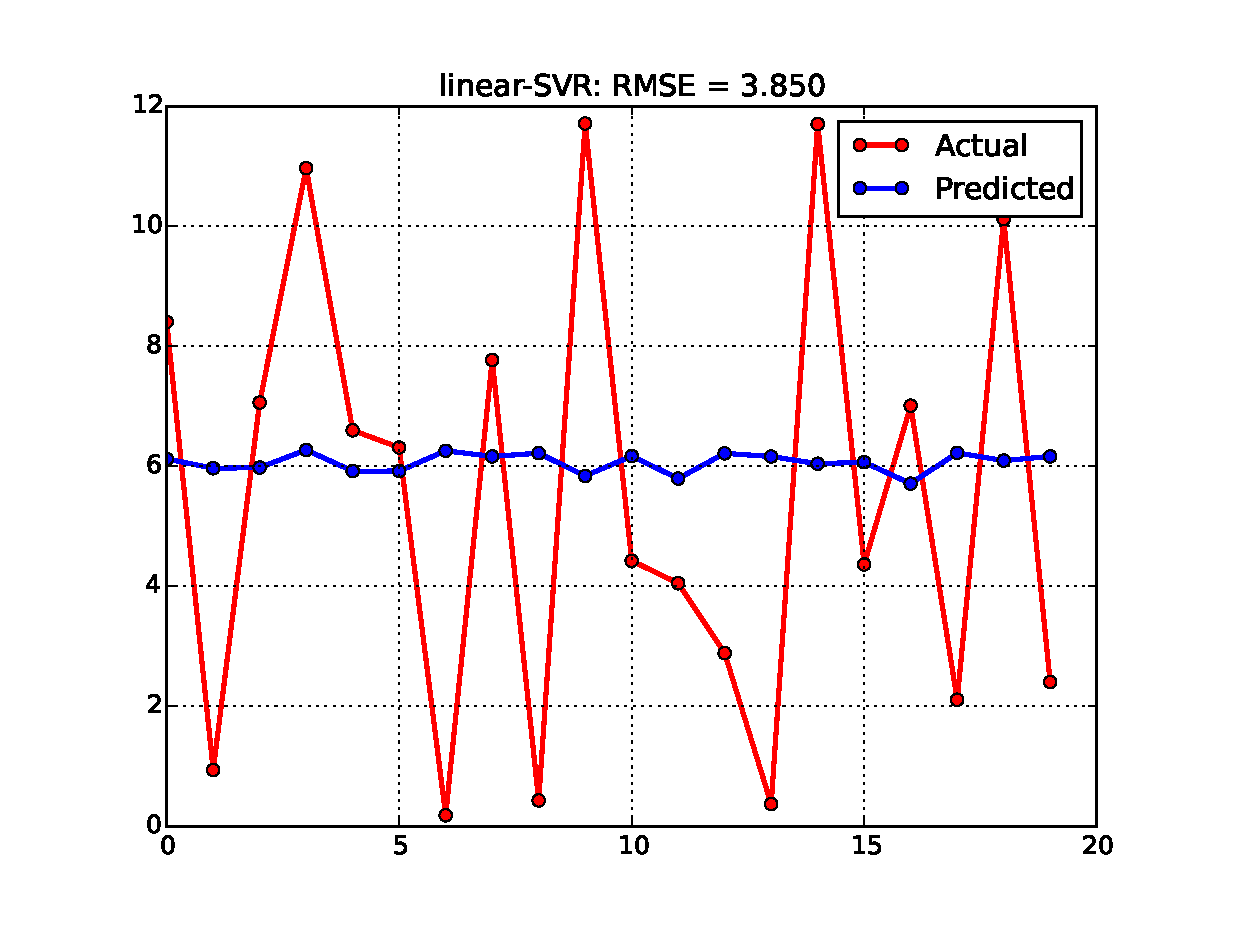
\includegraphics[width=\linewidth]{linear-SVR.eps}
\captionof{figure}{Linear kernel - Support Vector Regression}
\end{center}
\begin{center}
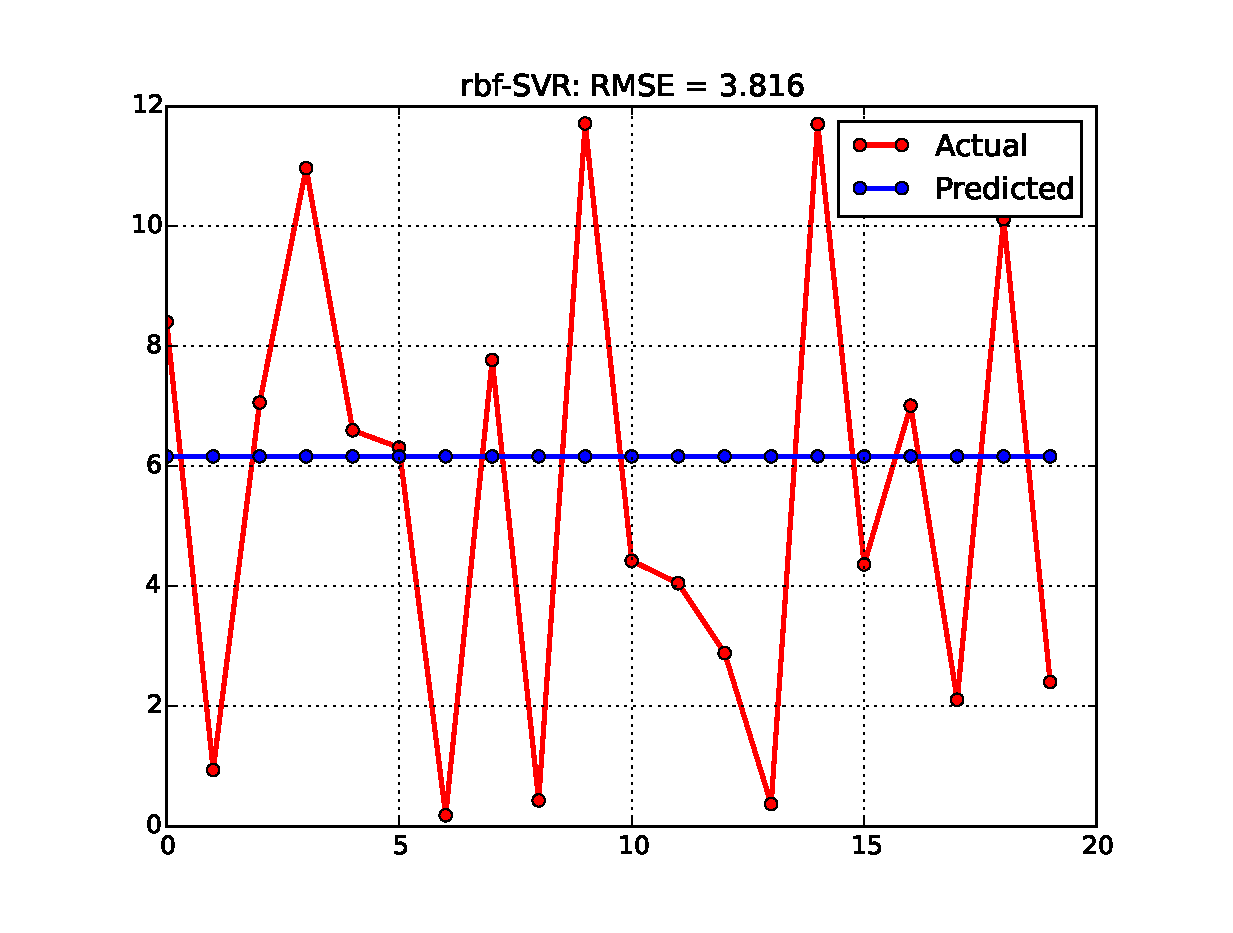
\includegraphics[width=\linewidth]{rbf-SVR.eps}
\captionof{figure}{RBF kernel - Support Vector Regression}
\end{center}
\begin{center}
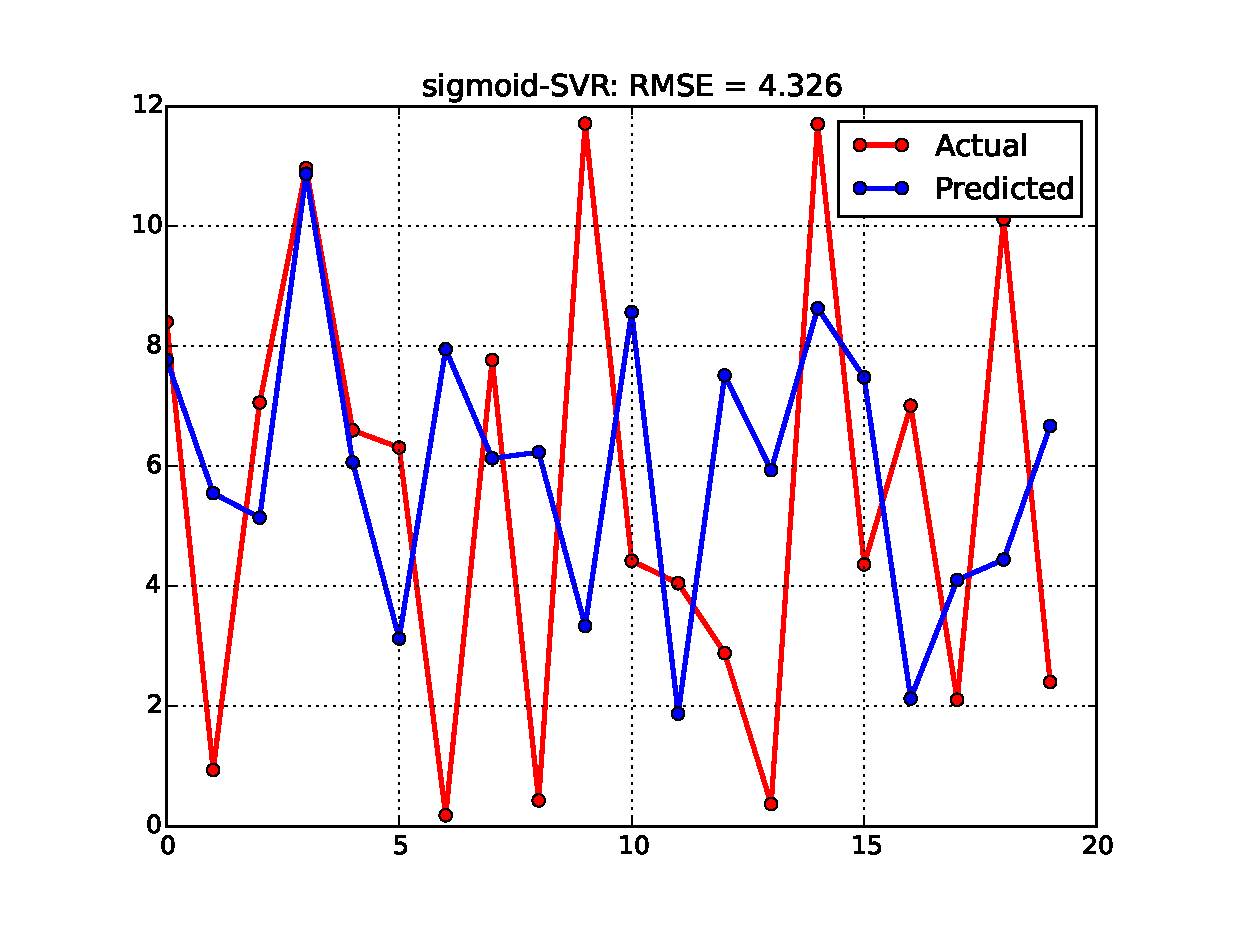
\includegraphics[width=\linewidth]{sigmoid-SVR.eps}
\captionof{figure}{Sigmoid kernel - Support Vector Regression}
\end{center}

\color{SaddleBrown} % SaddleBrown color for the conclusions to make them stand out

\section*{Conclusions}
Sigmoid kernel - Support Vector Regression has the strongest robust property.

\color{black}
\section*{Website}
\subsection*{Overview}
\begin{enumerate}
\item A fully functional hosted website, smartphone friendly and resizable to fit any size screen.
\item Displaying real time data, allow different filters to narrow down searching range.
\item Clean and neat UI design to introduce smart garbage recycle system from hardware to software, from sensors to backend server all the way to the database and frontend development.
\item Easy to check current status and history data of any garbage can at certain location.
\item Prediction for future garbage dectile.
\item  Information included: garbage can id, time, dectile.
\end{enumerate}
\subsection*{Architecture}
\begin{center}
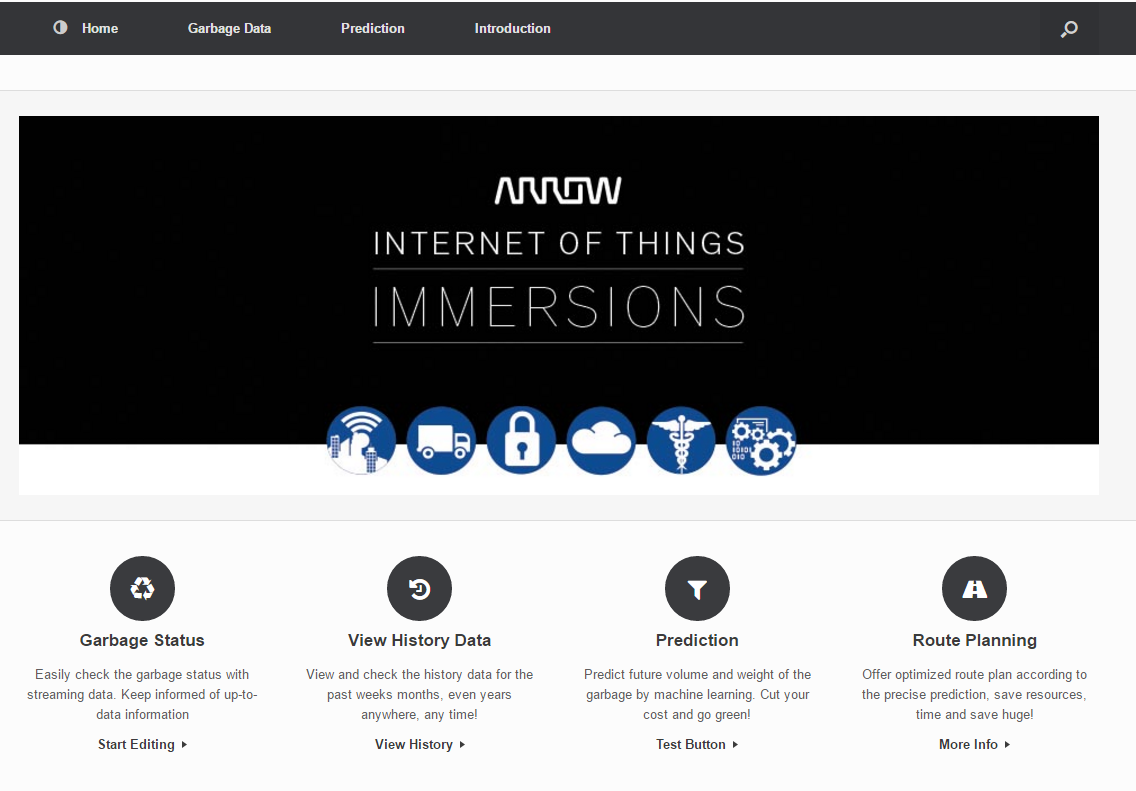
\includegraphics[width=\linewidth]{home.PNG}
\captionof{figure}{Homepage of smartgarbagerecycle.com}
\end{center}
\begin{center}
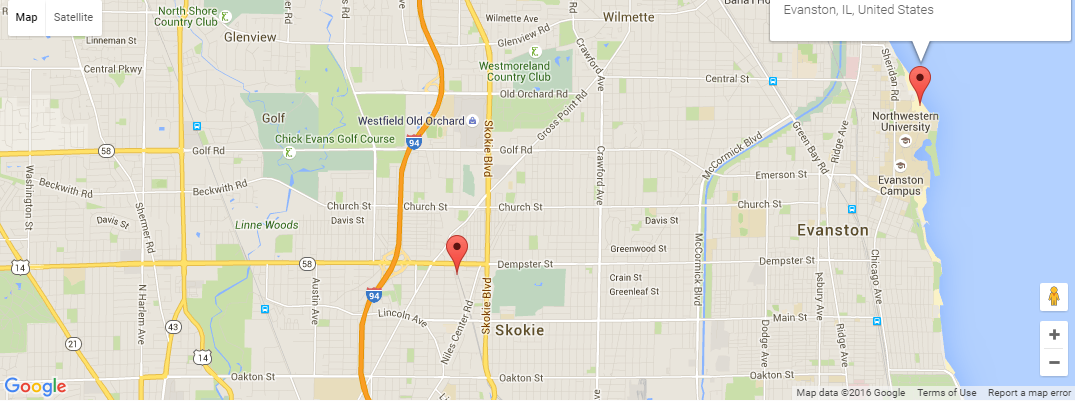
\includegraphics[width=\linewidth]{status.PNG}
\captionof{figure}{Garbage Status section of smartgarbagerecycle.com: Easily check the garbage status with streaming data. Keep informed of up-to-date information}
\end{center}
\begin{center}

\includegraphics[width=\linewidth]{database01.PNG}
\captionof{figure}{View History Data section of smartgarbagerecycle.com: Print out the search result into csv file, excel file or pdf file.}
\end{center}
\begin{center}
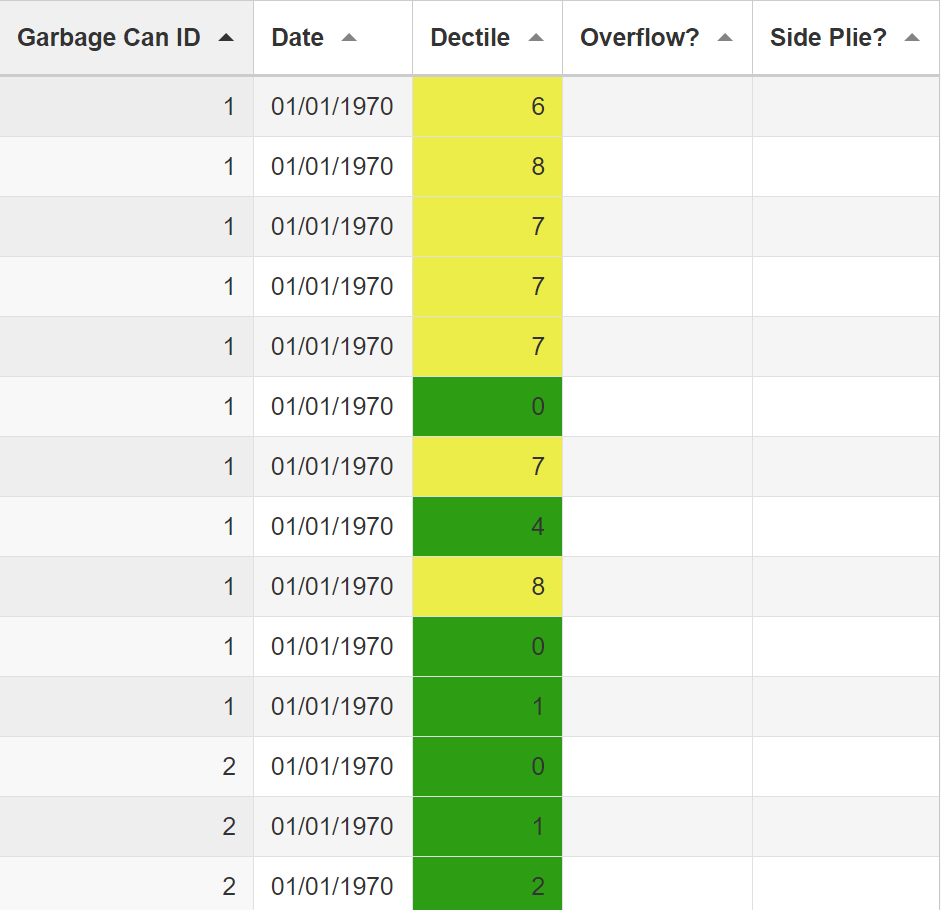
\includegraphics[width=\linewidth]{database02.PNG}
\captionof{figure}{View History Data section of smartgarbagerecycle.com: Review history garbage data according to garbage ID, time, and dectile}
\end{center}

\color{Black} % Set the color back to DarkSlateGray for the rest of the content

%----------------------------------------------------------------------------------------
%	FORTHCOMING RESEARCH
%----------------------------------------------------------------------------------------

\section*{Forthcoming Research}
\begin{enumerate}
\item Retrieve real-time data from database and showing different form of data visualization.
\item Making another layer on the current map and mark the garbage cans such that data could be directly checked on the map.
\item Improve the accuracy of prediction and combine the information from current recycle schedule, more collection data to do route planning. 
\end{enumerate}


\end{multicols}
\end{document}